\documentclass[a4paper,12pt]{article}
\usepackage[margin=0.7in]{geometry}
\usepackage{tikz}
\usepackage{float}
\usepackage{pdflscape}
\usetikzlibrary{positioning,arrows.meta,shapes.geometric,fit,calc}
\begin{document}

\section*{Report Generation and Exports}
\begin{figure}[H]\centering
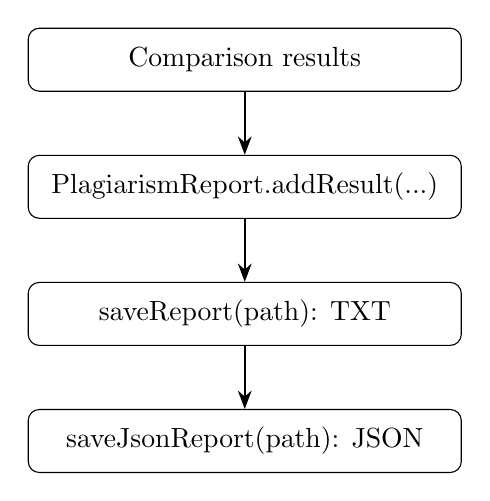
\begin{tikzpicture}[node distance=8mm, every node/.style={draw,rounded corners,align=center,minimum width=5.5cm,minimum height=8mm}, flow/.style={-{Stealth},thick}]
\node (n0) {Comparison results};
\node (n1) [below=of n0] {PlagiarismReport.addResult(...)};
\node (n2) [below=of n1] {saveReport(path): TXT};
\node (n3) [below=of n2] {saveJsonReport(path): JSON};
\draw[flow] (n0)--(n1);
\draw[flow] (n1)--(n2);
\draw[flow] (n2)--(n3);
\end{tikzpicture}
\textit{TXT/JSON are represented; CSV export was not found in the supplied source.}
\caption{Report Generation and Exports workflow.}\end{figure}
\end{document}
